\subsection{Big Data}
\begin{frame}{Mi az a Big Data?}
    \begin{columns}
        \begin{column}{0.5\textwidth}
            Large Synoptic Survey Telescope
            \begin{itemize}[<+->]
                \item Minden éjszaka feltérképezi a fél eget, ami
                \item 15 terabájt (TB) adatot termel.
                \item 10 év alatt 50 petabájt (1 PB = 1000 TB) nyers adat keletkezik,
                \item ami feldolgozva több, mint 100 PB lesz.
            \end{itemize}
            
            CERN
            \begin{itemize}[<+->]
                \item 2017. december: 1 PB adat közzététele (\href{https://home.cern/news/news/experiments/cms-releases-more-one-petabyte-open-data}{\textcolor{cyan}{CERN News}})
                \item Összesen $\sim$1,5 PB
            \end{itemize}
        \end{column}
        \begin{column}{0.5\textwidth}
            \centering
            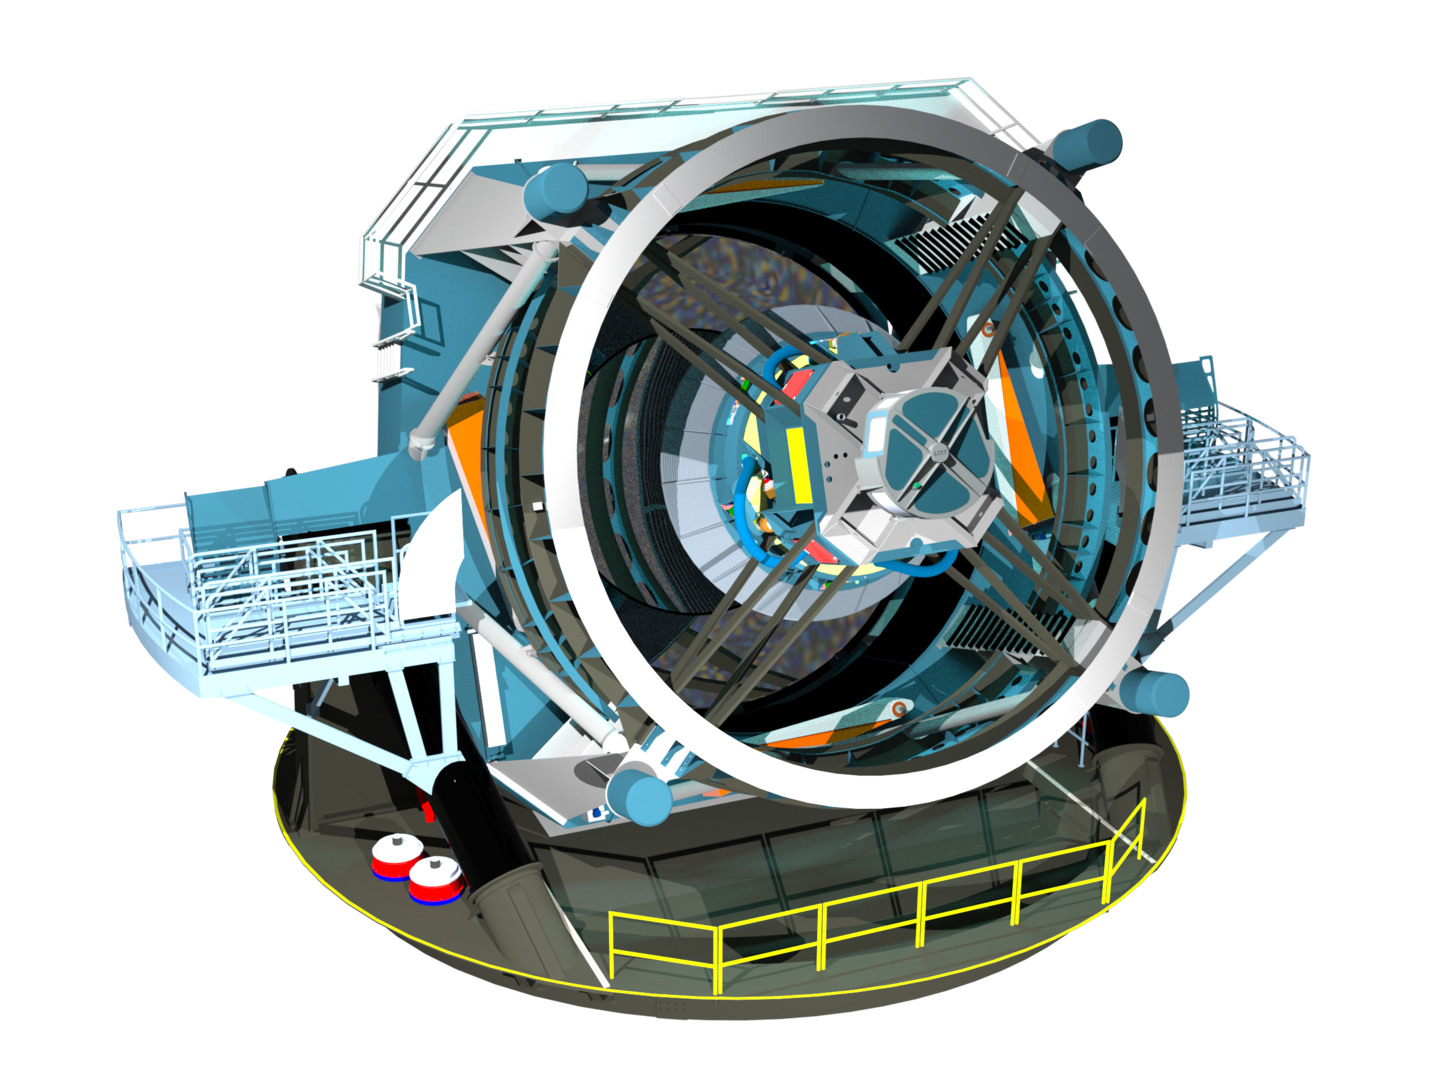
\includegraphics[height=0.4\textheight]{figures/lsst.png} \\ %0.13
            \tiny{Fotó: LSST}

            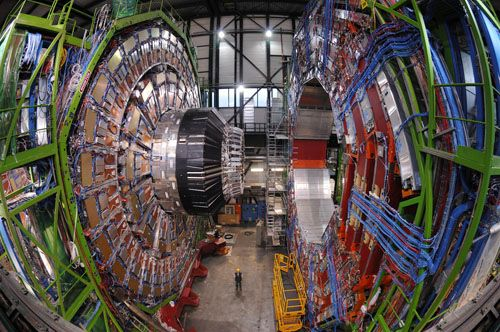
\includegraphics[height=0.4\textheight]{figures/cms.jpg} \\ %0.25
            \tiny{Fotó: CERN/CMS}
        \end{column}
    \end{columns}
\end{frame}

\begin{frame}{Mi az a Big Data?}
    \begin{block}{Mi az a Big Data?}
        Az az adatmennyiség, amit a hagyományos adatbáziskezelők már nem tudnak kezelni, mert túl nagy, gyorsan fel kell dolgozni és sok formában létezhet.
    \end{block}
    A Big Data 4V-je:
    \begin{itemize}
        \item Volume (Mennyiség)
        \item Velocity (Sebesség)
        \item Variety (Sokféleség)
        \item Veracity (Bizonytalanság)
    \end{itemize}
\end{frame}

\begin{frame}{Big Data - problémák és a megoldás}
    Problémák:
    \begin{itemize}
        \item Nincs ember, aki lépést tud tartani ekkora adatmennyiséggel
        \item A "hagyományos" adatfeldolgozó algoritmusok túl lassúak
        \item Változó minőségű adatok
        \item Adatvizualizáció problémás lehet ($d > 3D$)
    \end{itemize}
    
    Megoldás: mesterséges intelligencia
    \begin{itemize}
        \item Minimális emberi beavatkozás kell
        \item Jó alak- és mintafelismerők
        \item Gyorsak és pontosak (de ehhez dolgozni kell)
        \item Jól kidolgozott eszközök: {\it tensorflow}, {\it keras}, {\it pandas}, {\it scikit-learn}, {\it numpy}, {\it pytorch}\dots
    \end{itemize}
\end{frame}
